% Editable reconstruction; interpretation recorded in root.json.
% Shared standalone design for the editable figure reconstructions.
\documentclass[tikz,border=5pt,10pt]{standalone}
\usepackage[T1]{fontenc}
\usepackage[utf8]{inputenc}
\usepackage{newpxtext,newpxmath}
\usepackage[scaled=.94]{sourcesanspro}
\usepackage{pgfplots}
\pgfplotsset{compat=1.18}
\usetikzlibrary{arrows.meta,calc,positioning,decorations.pathreplacing,
  decorations.markings,patterns,matrix,shapes.geometric,fit,backgrounds,
  intersections,angles,quotes}
\definecolor{ink}{HTML}{203746}
\definecolor{accent}{HTML}{146C78}
\definecolor{muted}{HTML}{667780}
\definecolor{signalred}{HTML}{B94B44}
\color{ink}
\tikzset{>=Latex,line width=.8pt,
  every node/.style={font=\small},
  axis/.style={->,draw=muted,line width=.5pt},
  guide/.style={draw=muted,dashed,line width=.45pt},
  curve/.style={draw=accent,line width=1pt},
  marker/.style={circle,fill=accent,inner sep=1.5pt},
  labelbox/.style={fill=white,inner sep=2pt}}

\begin{document}

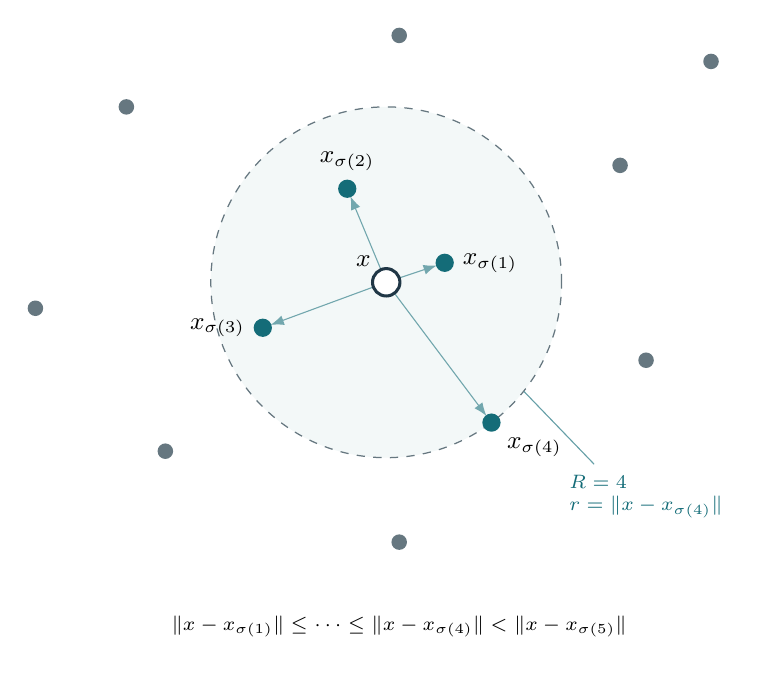
\begin{tikzpicture}[scale=1.65]
\fill[accent!5] (0,0) circle(1.35);
\draw[guide] (0,0) circle(1.35);
\foreach \x/\y/\i/\pos in {.45/.15/1/right,-.3/.72/2/above,-.95/-.35/3/left,.81/-1.08/4/below right}{
\draw[->,accent!60,shorten >=3pt] (0,0)--(\x,\y);
\fill[accent] (\x,\y) circle(2pt);
\node[\pos=3pt] at (\x,\y) {$x_{\sigma(\i)}$};}
\foreach \p in {(-2,1.35),(-1.7,-1.3),(.1,1.9),(1.8,.9),(2,-.6),(.1,-2),(2.5,1.7),(-2.7,-.2)}{\fill[muted] \p circle(1.7pt);}
\draw[ink,fill=white,line width=1.1pt] (0,0) circle(3pt);
\node[above left=3pt] at (0,0) {$x$};
\node[font=\scriptsize,accent,align=left] at (2,-1.65) {$R=4$\\$r=\|x-x_{\sigma(4)}\|$};
\draw[accent!65] (1.6,-1.4)--(1.06,-.84);
\node[font=\scriptsize] at (.1,-2.65) {$\|x-x_{\sigma(1)}\|\leq\cdots\leq\|x-x_{\sigma(4)}\|<\|x-x_{\sigma(5)}\|$};
\end{tikzpicture}
\end{document}
